\subsection{Telepítés}
Nincs szükség telepítésre.
\subsection{Futtatás}
A program java programozási nyelvben lett megírva, így a kifordított állomány egy jar file, melyet parancssorból az alábbi utasítással tudunk futtatni
\begin{lstlisting}
java -jar <filenev>
\end{lstlisting}
\subsection{Felhasznált technológiák}
A szakdolgozatomat eclipse fejlesztőkörnyezetben írtam, amelyet végül mavennel - build rendszer - fordítottam ki és csomagoltam be. A szakdolgozat felhasznál egy külső könyvtárat, amely a nyertes kiértékelési feladatát látja el. A programcsomagot meg kellett támogatni egy adatbázissal is - MySQL - , amely az adatok perzisztens tárolásáért felel. A programcsomag szerver-kliens architektúrában került implementálásra, amely tovább bomlik kliens oldalon MVC (Model-View-Controller) tervezési stílusra. A modulok közötti kommunikáció RMI Java API felhasználásával történik.
\subsection{Adatbázis séma}
\begin{figure}[h!]
  \caption{Adatbázis séma}
  \centering
    \includegraphics[width=0.5\textwidth]{user-documentation/images/db_scheme.png}
\end{figure}
\subsection{Modulok}
A programcsomag 6 fő modult tartalmaz
\begin{itemize}
  \item poker-server
  \item poker-client
  \item poker-shared
  \item poker-persist
  \item poker-model
  \item javapokertexasholdem
\end{itemize}
\begin{figure}[h!]
	\caption{Kliens modulra bontása}
	\centering
	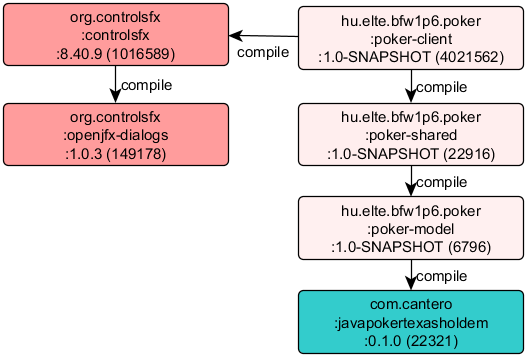
\includegraphics{user-documentation/images/poker-client-deps.png}
\end{figure}
\begin{figure}[h!]
	\caption{Szerver modulra bontása}
	\centering
	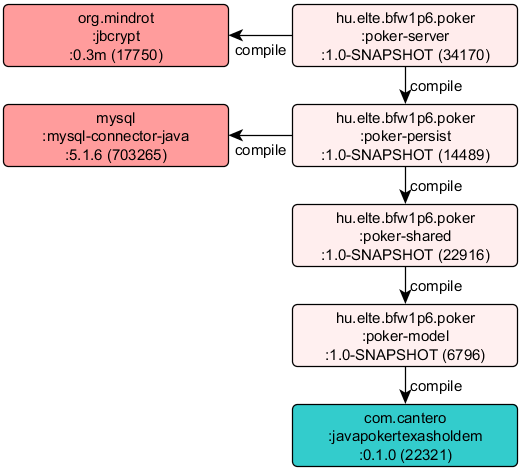
\includegraphics{user-documentation/images/poker-server-deps.png}
\end{figure}
A modulok közötti függőséget a ... ábra mutatja. A programcsomag két fő modulra bontható: poker-server és poker-client. A szerver a jelszavak titkosítására bcrypt eljárást alkalmaz, amelynek a biztonságát sózással növeli. Továbbá a szerver felhasznál még egy külső csomagot - mysql-connector-java -, amely az adatbázis kapcsolatért felel.
A poker-shared modul felel a szerver és a kliens jól definiált kommunikácójáért. A shared modul többek között tartalmazza a közös interfészeket, kivételeket és a póker utasítások megvalósítását.

\section{Tovább fejlesztési lehetőségek}
\begin{itemize}
\item Az adatbázis viszonylag alacsony absztrakciós szinten került implementására, azonban mivel néhány tábláról beszélhetünk csak, ezért igyekeztem elkerülni a keretrendszerek általi overheadet. Ugyanakkor ezen a ponton sokat fejlődhet a programcsomag, ha a későbbiek során esetlegesen bonyolultabban kellene modellezni a játékot adatbázis szempontjából. Például dialektusok - akár Liquibase (hivatkozás) - használata elfedheti a tényleges adatbázis-kezelő rendszer általánosságait, így eggyel magasabb szintre helyezhető a megvalósítás.
\item A felhasználói élményen sokat javíthat az animációk használata. A megjelenítés sokkal lágyabb, folyékonyabb lehetne Transition/Animation (bibliográfiába hivatkozás...) objektumok használatával.
\item Akár a komplett RMI architektúrát (JDK 1.1-ben jelent meg 18 éves technológia [a http meg 16...]) le lehetne váltani, és helyette REST szoftverarchitektúrát tenni, amely modernebb megjelenést (AngularJS, reszponzív design) és modernebb eszközöket vonna maga után.
\end{itemize}

%\begin{figure}[hbt]
%	\centering
%	\includegraphics[width=\linewidth, height=8cm]{db_scheme.png}
%	\caption{Adatbázis séma}
%	\label{fig:lol}
%\end{figure}

A \ref{fig:lol} képen látható az adatbázis séma.

\begin{tabular}{| l | c | r |}
\hline
  1 & 2 & 3 \\ \hline
  4 & 5 & 6 \\ \hline
  7 & 8 & 9 \\ \hline
\end{tabular}

\clearpage
